\section{Payload and Payload--Range Efficiency}
\label{sec:payload-range-efficiency}

The payload efficiency and payload--range efficiency plots were made by keeping the
final aircraft geometry fixed and sweeping the mission payload and fleet size. The
fixed design values were loaded from \texttt{final\_design\_values.json}; therefore
the wing span, aspect ratio, empty mass, battery mass, tail geometry, drag terms,
maximum lift coefficient, drivetrain efficiency, and available thrust were not
re-optimized during the sweep. This means that the plots show how the selected final
design performs away from its nominal design point, rather than showing a new
optimum aircraft for every payload.

For each number of drones, \(n=3,4,5,6\), the total payload \(m_p\) was varied. For
each payload case, the sizing model recalculates the required lift coefficient and
the induced drag of the wing. The total drag coefficient used in the sweep is
\begin{equation}
    C_D =
    C_{D,\mathrm{fixed}}
    + k C_L^2
    + C_{D,\mathrm{payload}}
      \frac{S_\mathrm{payload}}{n S_w},
\end{equation}
where \(C_{D,\mathrm{fixed}}\) contains the non-induced drag of the aircraft without
the payload, \(kC_L^2\) is the induced drag contribution, and the last term accounts
for the drag of the suspended payload shared over the total wing area of the fleet.
The drag per drone is then
\begin{equation}
    D = C_D q S_w .
\end{equation}
The electrical energy required per kilometre for the full fleet is calculated from
this drag force as
\begin{equation}
    e_\mathrm{km} =
    \frac{nD}{3.6\eta_\mathrm{drive}},
\end{equation}
where \(\eta_\mathrm{drive}\) is the drivetrain efficiency. This expression follows
from \(P=nDV/\eta_\mathrm{drive}\) and a flight time of \(1000/V\) seconds per
kilometre.

Each payload case is only accepted if it satisfies the aerodynamic and propulsion
limits. In particular,
\begin{equation}
    C_L \leq C_{L,\max}, \qquad
    D \leq T_\mathrm{max}.
\end{equation}
After this check, the battery-limited cruise range is found from
\begin{equation}
    R_\mathrm{bat} =
    \frac{
        nE_{\mathrm{usable,drone}} - E_{\mathrm{climb,fleet}}
    }{e_\mathrm{km}},
\end{equation}
where \(E_{\mathrm{usable,drone}}\) is obtained from the battery mass and depth of
discharge of the final design. The climb energy is estimated for each payload case
using the same climb rate and climb duration as the sizing model.

The payload--range efficiency figure is made by adding a second sweep over the
required mission range up to \(50~\mathrm{km}\). For each point \((m_p,R)\) on the
grid, the script compares all
feasible fleet sizes. A fleet size is a candidate only if its battery-limited range
is at least the required range. Among the candidates, the selected option is the one
with the lowest total energy consumption per kilometre. If no fleet size can carry
the payload over the required range, the point is marked as infeasible.

\begin{figure}[htbp]
    \centering
    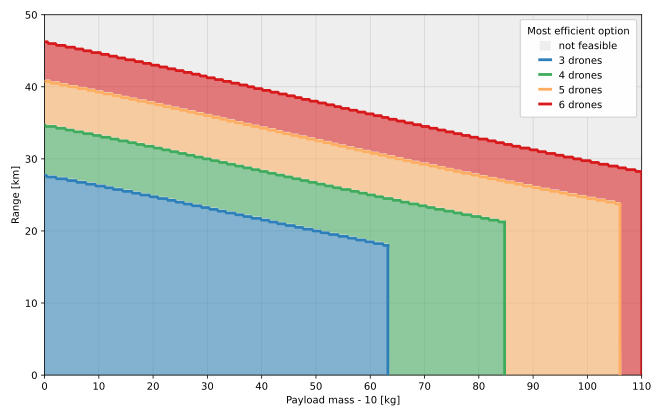
\includegraphics[width=0.85\textwidth]{payload_range_efficiency.svg}
    \caption{Best fleet size as a function of payload mass and required range. The
    coloured regions show the lowest-energy feasible number of drones, while the
    grey region indicates combinations that cannot be flown with the available
    battery, lift, or thrust.}
    \label{fig:payload-range-efficiency}
\end{figure}

Figure~\ref{fig:payload-range-efficiency} shows that low payload and low range
missions are most efficiently completed with three drones. As the payload increases,
additional drones become favourable because the payload is distributed over more
airframes, reducing the required lift and drag per drone. The boundary lines also
show the maximum battery-limited range for each fleet size. The figure therefore visualizes the main
trade-off in the system: adding drones increases the payload capability, but it also
adds aircraft drag and energy consumption, so the most efficient fleet size depends
on both payload mass and required range.

\begin{figure}[htbp]
    \centering
    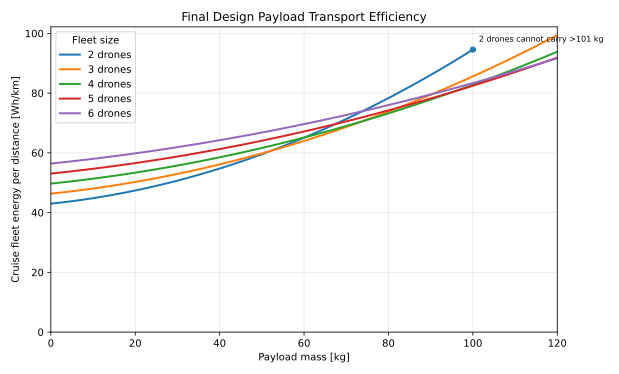
\includegraphics[width=0.75\textwidth]{payload_efficiency.svg}
\caption{Payload efficiency sweep showing how the energy consumption changes
    with payload for the feasible part of each fleet-size curve.}
    \label{fig:payload-efficiency}
\end{figure}

The payload efficiency plot in Figure~\ref{fig:payload-efficiency} provides the
one-dimensional version of the same calculation. It shows the increase in energy
required per kilometre as the carried payload is increased. The payload--range plot
then extends this result by comparing the available battery energy with the mission
range requirement and selecting the best feasible fleet size at each grid point.
